% Created 2020-07-27 Mon 16:01
% Intended LaTeX compiler: pdflatex
\documentclass[presentation]{beamer}
\usepackage[utf8]{inputenc}
\usepackage[T1]{fontenc}
\usepackage{graphicx}
\usepackage{grffile}
\usepackage{longtable}
\usepackage{wrapfig}
\usepackage{rotating}
\usepackage[normalem]{ulem}
\usepackage{amsmath}
\usepackage{textcomp}
\usepackage{amssymb}
\usepackage{capt-of}
\usepackage{hyperref}
\usetheme{UoB}
\author{Mark Blyth}
\date{\textit{[2020-07-27 Mon]}}
\title{Deep learning: An Introduction for Applied Mathematicians}
\hypersetup{
 pdfauthor={Mark Blyth},
 pdftitle={Deep learning: An Introduction for Applied Mathematicians},
 pdfkeywords={},
 pdfsubject={},
 pdfcreator={Emacs 26.3 (Org mode 9.1.9)}, 
 pdflang={English}}
\begin{document}

\maketitle

\section{{\bfseries\sffamily TODO} Background}
\label{sec:org1544ad8}


\section{Network design}
\label{sec:orge45367f}
\begin{frame}[<+->][label={sec:org565ed6f}]{Background}
\begin{definition}[Neural network]
A nonlinear model that's general enough to fit most data
\end{definition}

\vfill
\begin{itemize}
\item Take input vectors \(\mathbf{x}_i\)
\item Take output vectors \(\mathbf{y}_i\)
\item Fit some nonlinear model \(\mathbf{y} = f(\mathbf{x})\)
\end{itemize}
\end{frame}

\begin{frame}[label={sec:org37b6e12}]{Drilling site example}
\begin{itemize}
\item Input data: \(\mathbf{x}_i = (u_i, v_i)\), oil well location
\item Output data: \(y_i\in\{0,1\}\), success or failure
\item Learn some nonlinear model mapping locations to drill successes
\end{itemize}
\end{frame}

\begin{frame}[<+->][label={sec:org2ea6b2d}]{Model form}
How do we create a nice general model?
\vfill
\begin{itemize}
\item A neural network is just a convenient representation of `stringed nonlinearities'
\item Take a simple nonlinearity, eg. sigmoid \(\sigma(x)\)
\item String a load of them together
\begin{itemize}
\item \(f(x) = \sigma(\sigma(\dots\sigma(x)\dots)\)
\end{itemize}
\item More useful: can shift mean, scale with a linear transform \(\sigma(wx + b)\)
\begin{itemize}
\item \(f(x) = \sigma(b + w\sigma(b + w\sigma( \dots \sigma(b + w\sigma(x)) \dots )\)
\end{itemize}
\item Fit the model
\begin{itemize}
\item Find appropriate values for each \(w, b\)
\end{itemize}
\end{itemize}
\end{frame}

\begin{frame}[label={sec:orgdcec713}]{Why `neural network'?}
\begin{itemize}
\item We can represent the equation nicely as a graph
\end{itemize}
\vspace{-.3cm}
\begin{center}
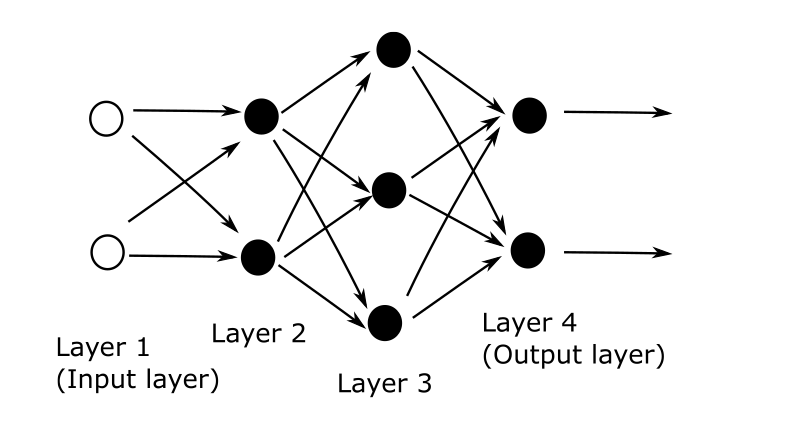
\includegraphics[height=.7\textheight]{./net.png}
\end{center}      
\vspace{-.7cm}
\begin{itemize}
\item Information flows forward through the graph much like it does through the brain
\end{itemize}
\end{frame}


\begin{frame}[<+->][label={sec:orgb9cb929}]{Model form}
\begin{itemize}
\item Node inputs = weighted sum of previous layer's outputs
\begin{itemize}
\item Vector form: \(\mathbf{i}_k = W_k \mathbf{o}_{k-1} + \mathbf{b}_k\)
\end{itemize}
\item Node output = sigmoid of inputs
\begin{itemize}
\item \(\mathbf{o}_k = \sigma(\mathbf{i}_k)\)
\end{itemize}
\item Inputs can be efficiently computed with some linear algebra
\item Much neater representation than `stringed nonlinearities'
\end{itemize}
\end{frame}

\begin{frame}[<+->][label={sec:orga0f0402}]{Why does this work?}
Loosely speaking\ldots{}
\vfill
\begin{itemize}
\item Having lots of \(W_k\), \(b_k\) gives us a very general model
\item We can fit the data by selecting \(W\), \(b\) to minimise the error \(\sum\| f(\mathbf{x}_i - \mathbf{y}_i \|^2\)
\item Universal approximator!
\end{itemize}
\end{frame}


\section{Network training}
\label{sec:org103eaae}
\begin{frame}[<+->][label={sec:orgfa6ccb1}]{Network training}
We now have a model; how do we fit it?

\begin{definition}[Gradient descent]
Optimisation method that iteratively updates parameters with a most-improving step
\end{definition}

\begin{itemize}
\item Like a massless ball rolling down a hill
\begin{itemize}
\item Travels in the direction of greatest slope
\item Reaches a flat bit eventually
\end{itemize}
\item Flat bit means cost stops changing
\begin{itemize}
\item Could be a good fit, could be a saddle or local minimum
\end{itemize}
\end{itemize}
\end{frame}

\begin{frame}[<+->][label={sec:orge6dcc42}]{Stochastic gradient descent}
\begin{itemize}
\item Let \(\mathrm{cost}_p = \sum_i \| f_p(\mathbf{x}_i) - \mathbf{y}_i\|^2\)
\item Iteratively let \(p_{i+1} = p_i - \eta \frac{\partial \mathrm{cost}}{\partial p_i}\)
\begin{itemize}
\item Alternatively, calculate the cost over some `minibatches' and perform iterations on these
\end{itemize}
\item How do we find \(\frac{\partial \mathrm{cost}}{\partial p_i}\)?
\end{itemize}
\end{frame}

\begin{frame}[label={sec:orgc8edd97}]{Backprop}
\begin{definition}[Backpropagation]
A method for finding cost-function gradient, given
\begin{itemize}
\item a cost function
\item a nonlinearity
\item a network topology
\end{itemize}
\end{definition}

\vfill
Backprop is the core of NN training!
\end{frame}

\begin{frame}[<+->][label={sec:orga77c89b}]{How does backprop work?}
For a single input\ldots{}
\begin{itemize}
\item How does cost function change with last layer's outputs?
\begin{itemize}
\item \(\frac{\partial\mathrm{cost}}{\partial \mathrm{output}} = 2\|f(\mathbf{x}_i) - \mathbf{y}_i\|\)
\end{itemize}
\item How does \(i\)th layer output change with \(i\)th layer input?
\begin{itemize}
\item \(\frac{\partial\mathrm{output}}{\partial\mathrm{input}} = \sigma'(\mathrm{input})\)
\end{itemize}
\item How does \(i\)th layer input change with \(i\)th layer weights, biases?
\begin{itemize}
\item \(\frac{\partial \mathrm{input}}{\partial \mathrm{weights}} = (i-1)\mathrm{'th~layer~output}\)
\item \(\frac{\partial \mathrm{input}}{\partial \mathrm{biases}} = 1\)
\end{itemize}
\item Can find cost function gradient by chain-ruling these all together
\item Can sum the resulting gradient across the full minibatch
\end{itemize}
\end{frame}


\begin{frame}[<+->][label={sec:orgf0a3a47}]{Backprop results}
Backprop gives us an easy way to compute \(\frac{\partial \mathrm{cost}}{\partial \mathrm{weights}}\) and \(\frac{\partial \mathrm{cost}}{\partial \mathrm{biases}}\)
\vfill
\begin{itemize}
\item Forward pass: find each node's inputs and outputs
\item Backward pass:
\begin{itemize}
\item Relate last layer's output to cost function gradient
\item Relate each previous layer's outputs, weights, biases to next layer's error
\item Relate next layer's error to cost function gradient
\end{itemize}
\item Propagates errors backward through the network
\end{itemize}
\end{frame}

\section{ConvNets}
\label{sec:org19e83bf}
\begin{frame}[label={sec:org079c9bb}]{Convolutional neural networks}
\begin{itemize}
\item Visual cortex has a `receptive field'
\item CNN mirror this with local kernel transforms
\item Convolutional layers automatically extract features
\item Allows NNs to efficiently manipulate high-dimensional data
\end{itemize}
\end{frame}

\section{Practical aspects}
\label{sec:org1ab8d8e}
\begin{frame}[label={sec:org4736d7e}]{Practical aspects}
\begin{definition}[Overfitting]
Representing the training data too closely, and losing the ability to generalise
\end{definition}
\end{frame}

\begin{frame}[<+->][label={sec:org87d9b57}]{Costs and activations}
\begin{itemize}
\item We don't have to use sigmoids
\begin{itemize}
\item ReLU: linear activation with positive support
\item Alternative: small gradient for negative numbers, large gradient for positive numbers
\end{itemize}
\item We don't have to use residuals
\begin{itemize}
\item Softmax-log-loss
\end{itemize}
\end{itemize}
\end{frame}

\section{Next paper}
\label{sec:org1871240}
\section{Discussion}
\label{sec:orgce99ca9}
\begin{frame}[label={sec:orgb2d8594}]{The essence of ML}
\begin{itemize}
\item Machine learning sounds flashy and cool; it's just big statistics
\item Large-scale model definitions and cost-function-fitting
\end{itemize}
\end{frame}

\begin{frame}[label={sec:orge8f2e22}]{Section 8 discussion points}
\begin{itemize}
\item Why use NNs?
\begin{itemize}
\item When do other methods generalise better?
\end{itemize}
\end{itemize}
\end{frame}
\begin{frame}[label={sec:org01d51af}]{Section 8 discussion points}
\begin{itemize}
\item How robust are the results?
\begin{itemize}
\item Do small input changes matter much? Should they?
\end{itemize}
\end{itemize}
\end{frame}
\begin{frame}[label={sec:org3b66f80}]{Section 8 discussion points}
\begin{itemize}
\item What's a sensible nonlinearity?
\begin{itemize}
\item Is there any reason to choose ReLU over sigmoids?
\end{itemize}
\end{itemize}
\end{frame}
\begin{frame}[label={sec:orgf64a65a}]{Section 8 discussion points}
\begin{itemize}
\item What topology do we need?
\begin{itemize}
\item How many hidden layers? How big?
\end{itemize}
\end{itemize}
\end{frame}
\begin{frame}[label={sec:org242c133}]{Section 8 discussion points}
\begin{itemize}
\item Can we regularise?
\begin{itemize}
\item Reduce overfitting by penalising model complexity
\end{itemize}
\end{itemize}
\end{frame}
\begin{frame}[label={sec:orgc156a9e}]{Section 8 discussion points}
\begin{itemize}
\item Explainability
\begin{itemize}
\item \emph{Why} should NNs give good results? Why do they give the results they do?
\end{itemize}
\end{itemize}
\end{frame}

\begin{frame}[label={sec:org76a12df}]{Discussion}
\begin{itemize}
\item Why use NNs vs. another method?
\item What topology do we need?
\item What's a sensible nonlinearity?
\item How robust are the results, and how much do we care?
\item Can we regularise?
\item Explainability -- how much do we trust the results?
\item How much can we actually learn from a black box?
\item How much data is enough data?
\item What are the applications to nonlinear dynamics?
\end{itemize}
\end{frame}

\begin{frame}[label={sec:org0e42c05}]{Next paper}
Someone to lead?
\vfill
Suggestion: Heinonen, Markus, et al. "Learning unknown ODE models with Gaussian processes." arXiv preprint arXiv:1803.04303 (2018).
\end{frame}
\end{document}
